\chapter{Grundlagen}\label{chap:Grundlagen}
\section{Bevölkerungsdichte}
Die Bevölkerungsdichte eines Gebietes $\rho_{Gebiet}$ wird berechnet, indem die Anzahl der Einwohner im Gebiet $n_{Einwohner im Gebiet}$ durch die Fläche des Gebiets $A_{Gebiet}$ geteilt wird:
\begin{equation}
    \rho_{Gebiet} = \frac{n_{Einwohner im Gebiet}}{A_{Gebiet}}
\end{equation}
\section{7-Tages-Inzidenz}
\todo{soll ich die 7-Tages Inzidenz und die Bevölkerungsdichte hier oder in der Vorgehensweise erklären?}
\section{Susceptible-Infectious-Removed Modell}
Ein Weg zur Beschreibung der Pandemie bietet das SIR Modell \autocite{SIR}. Dieses Modell teilt die Mitglieder einer Menschengruppe in eine der drei folgenden Kategorie ein und ermöglicht es, die zeitliche Entwicklung einer Pandemie übersichtlich darzustellen:
\begin{itemize}
    \item \glqq{}susceptible\grqq{}: Menschen, welche angesteckt werden können.
    \item \glqq{}infectious\grqq{}: Infizierte Menschen, welche weitere Menschen anstecken können. Werden auch als "die aktiven Fälle" bezeichnet.
    \item \glqq{}recovered\grqq{}: Menschen, welche in die Kategorie \glqq{}infectious\grqq{} fielen und\\
    nun immun gegen die Krankheit sind. (Hierzu zählen auch Verstorbene)
\end{itemize}
Hierbei werden die Neuansteckungen ausgehend von einem infizierten Menschen mit der Reproduktionszahl $R$ beschrieben. Formal ist die Reproduktionszahl $R$ definiert durch die durchschnittliche Anzahl an infizierten Menschen pro Fall \autocite{ReZahl}.
%weitere Erklärung von R_0 siehe Fabians erste Einleitungsseite


\section{Korrelationsanalyse mithilfe einer Faltung}\label{sec:BeschreibungKorrelationsanalyse}

Um festzustellen, ob die 7-Tages-Inzidenzen einiger Landkreise im Vergleich zu anderen Landkreisen eher voraus- oder nacheilen, wird in diesem Fall eine \glqq{}Faltung\grqq{} verwendet \autocite{Korrelation}.

Bei diskreten Werten, aufgeteilt in zwei Zeitserien $X$ und $Y$, wie in diesem Fall, lässt sich eine Faltung sehr einfach umsetzen:
Für eine zeitliche Verschiebung $\tau$ wird mit jedem Wert $x_i$ zum jeweiligen Zeitpunkt $t_i$ aus der ersten Zeitserie mit dem zugehörigen Wert $y_i$ aus der zweiten Zeitserie eine Produkt gebildet. Der zugehörige Wert aus der zweiten Zeitserie entspricht hierbei dem Zeitpunkt $t$ des Wertes der ersten Zeitserie plus die gewählte Verschiebung $\tau$. Sollte dieser zweite Wert nicht existieren, wird kein Produkt gebildet.

Für jede zeitliche Verschiebung $\tau$, für die mindesten ein Produkt gebildet wird, werden alle möglichen Produkte aufsummiert.

Somit ergibt sich \autoref{eq:Korrelation}, mit $n := $ Länge von $X$ und wenn $y_{i+\tau} \not\in Y$, dann $y_{i+\tau} := 0$:
\begin{equation}\label{eq:Korrelation}
    c(\tau) = \sum_{i=1}^n x_i\cdot y_{i+\tau}
\end{equation}


Bildlich gesprochen wird die zweite Zeitserie an der ersten Zeitserie vorbeigeschoben, beginnend an dem Punkt, an dem ausschließlich das erste Element der ersten Zeitserie mit dem letzten Element der zweiten Zeitserie multipliziert wird. Dies ist beispielhaft mit den Folgen $[1,2,3,2]$ und $[5,7,5,1]$ in \autoref{fig:Korrelation Beispiel} dargestellt.

\begin{figure}
    \centering
    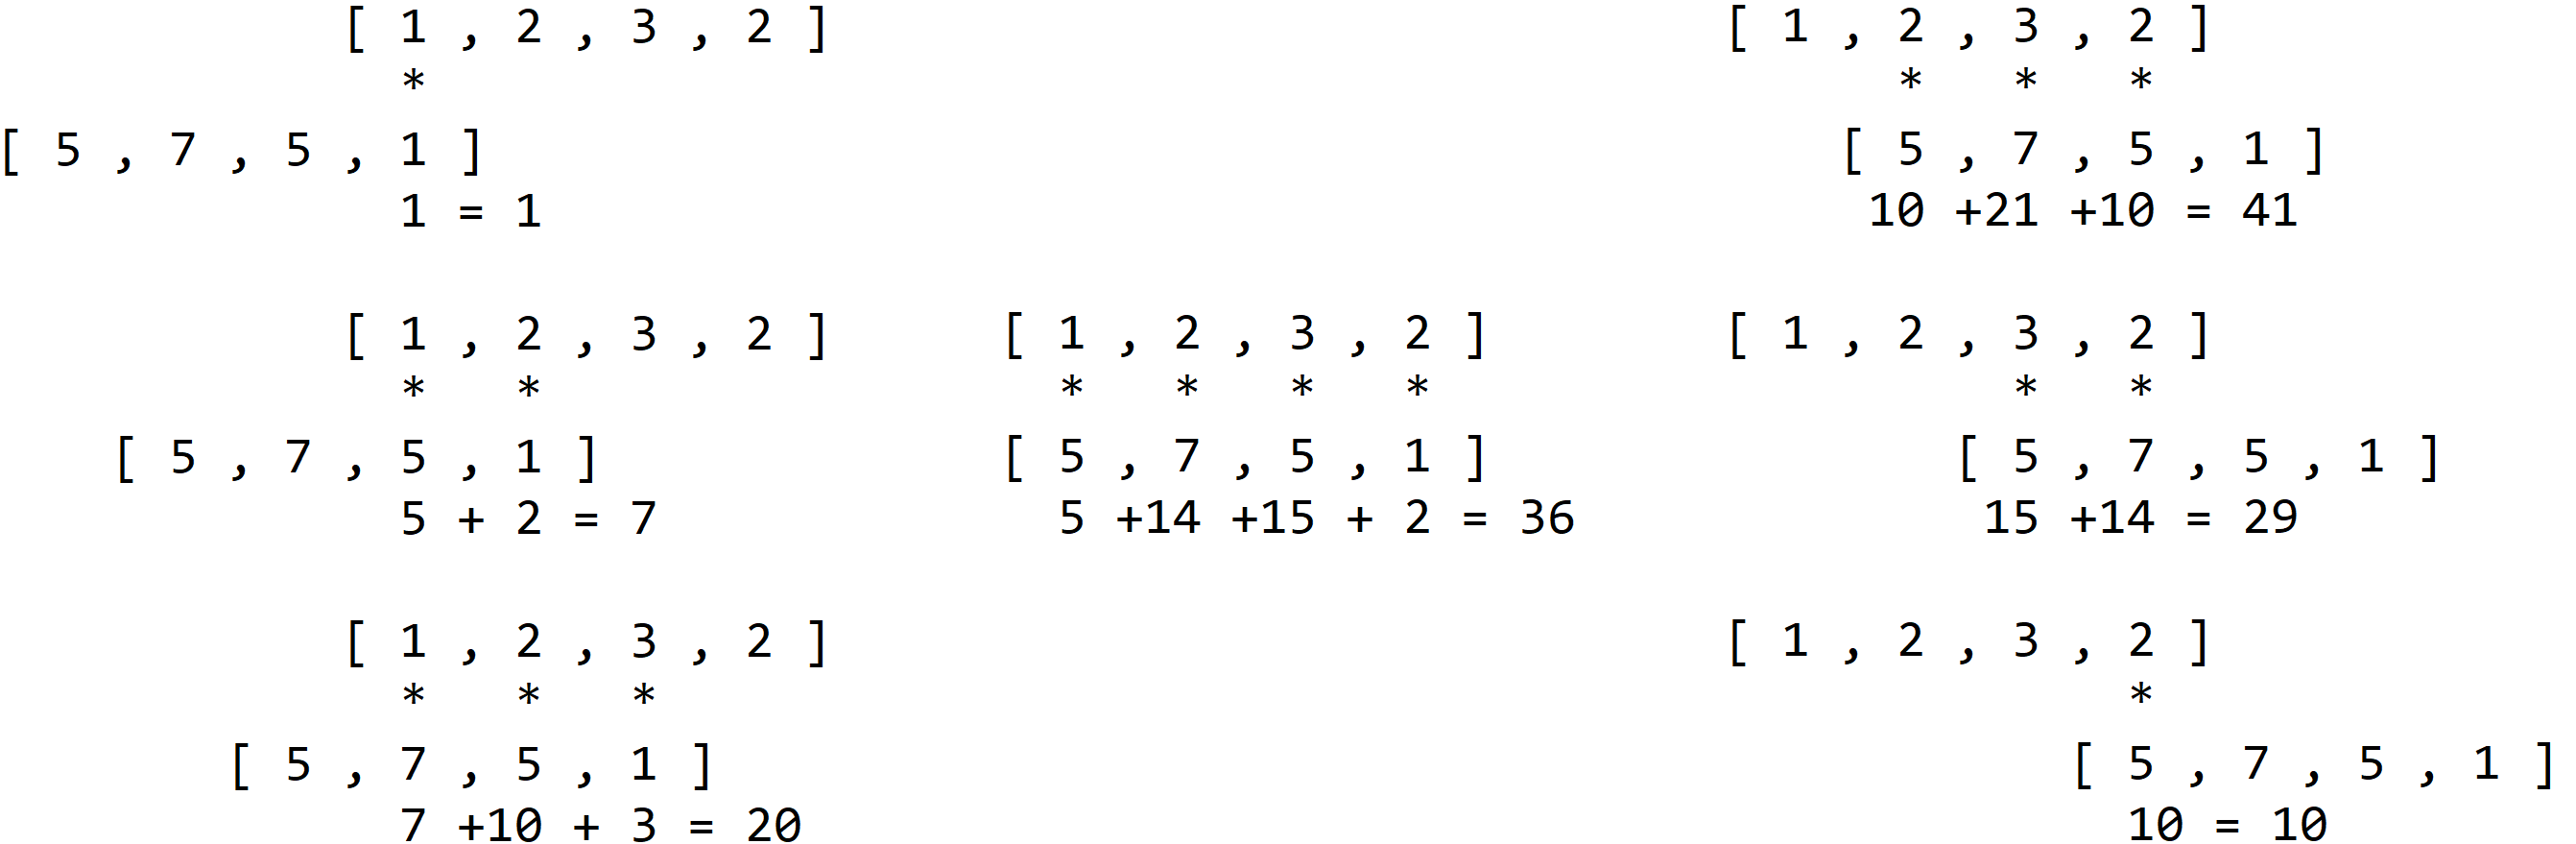
\includegraphics[width=\textwidth]{figures/Korrelation.png}
    \caption{Beispielhafte Darstellung einer Faltung anhand der Folgen $[1,2,3,2]$ und $[5,7,5,1]$. Auf der linken Seite hinter dem Gleichheitszeichen von oben nach unten die Korrelationswahrscheinlichkeiten für die negativen Verschiebungen $\tau=-3$, $\tau=-2$ und $\tau=-1$. Entsprechend in der Mitte bei keine Verschiebung ($\tau=0$) und rechts für die positiven Verschiebungen $\tau=1$, $\tau=2$ und $\tau=3$}
    \label{fig:Korrelation Beispiel}
\end{figure}

Da in diesem Beispiel jedoch die Landkreise mit höheren Werten scheinbar eine größere Korrelation aufweisen und die kleineren Verschiebungen übergewichtet werden, da ihre Summe aus mehr Produkten besteht, müssen die Werte noch skaliert werden.
Um die Landkreise mit allgemein größeren Werte anzupassen, wird durch die Autokorrelation mit keiner zeitlichen Verschiebung
geteilt, somit ergibt sich für die neuen Werte immer eine Autokorrelationswahrscheinlichkeit von eins bei keiner zeitlichen Verschiebung.
\begin{equation}\label{eq:Korrelation}
    c(\tau) =\sum_{i=1}^n \frac{x_i}{\sqrt{\sum_{j=1}^n x_j^2}}
    \frac{y_{i+\tau}}{\sqrt{\sum_{j=1}^n y_j^2}}= 
    \frac{\sum_{i=1}^n x_i\cdot y_{i+\tau}}{\sqrt{\sum_{i=1}^n x_i^2}\sqrt{\sum_{i=1}^n y_i^2}}
\end{equation}

Da bei der Faltung bei größeren Verschiebungen zudem weniger Produkte aufsummiert werden, muss bei jeder Summe durch die Anzahl der aufsummierten Produkte geteilt werden. Da jede Zeitserie gleich lang ist, in diesem Fall $n$ Elemente, ergibt sich folgende Gleichung, wobei die Anzahl der Produkte $m$ der Länge der Zeitserie $n$ minus den Betrag der Verschiebung $\vert\tau\vert$ entspricht:
\begin{equation}\label{eq:Korrelation}
    c(\tau) =\frac{n}{m} \frac{\sum_{i=1}^n x_i\cdot y_{i+\tau}}{\sqrt{\sum_{i=1}^n x_i^2}\sqrt{\sum_{i=1}^n y_i^2}}=
    \frac{n}{n-\vert\tau\vert} \frac{\sum_{i=1}^n x_i\cdot y_{i+\tau}}{\sqrt{\sum_{i=1}^n x_i^2}\sqrt{\sum_{i=1}^n y_i^2}}
\end{equation}

Zudem wird von jedem Wert der Zeitserie $x_i$ der Mittelwert $\overline x = \frac{1}{n}\sum_{i=1}^n x_i$ abgezogen, dadurch lassen sich Antikorrelationen feststellen: Wenn beispielsweise die Anzahl der COVID-19 Infektionen eines Landkreises zu einem Zeitpunkt überdurchschnittlich schnell wächst, also die 7-Tages-Inzidenz minus den Mittelwert der 7-Tages-Inzidenzen positiv ist, und das andere Edukt aus der anderen Zeitserie negativ ist, also in dem anderen Landkreis die Anzahl der COVID-19 Infektionen unterdurchschnittlich schnell wächst, ergibt sich ein negatives Produkt, da die Situation in dem einen Landkreis verhältnissmäßig ruhig wirkt, während die Situation im anderen Landkreis schneller als üblich kritisch wird. Ergibt die Summe aus all den Produkten einer Faltung eine negative Zahl, scheint die 7-Tages Inzidenz des einen Landkreises langsam zu steigen, wenn die 7-Tages Inzidenz des anderes Landkreises schnell zu steigen, dies wird hier Antikorrelation genannt.

\begin{equation}\label{eq:Korrelation}
    c(\tau) =\frac{n}{m}
    \frac{\sum_{i=1}^n (x_i-\overline x)\cdot (y_{i+\tau}-\overline y)}{\sqrt{\sum_{i=1}^n (x_i-\overline x)^2}\sqrt{\sum_{i=1}^n (y_i-\overline y)^2}}
\end{equation}
\todo{Quelle}
\section{Durchschnitt, Farbgebung und Skalierung}\label{sec:Durchschnitt, Farbgebung und Skalierung}
Um schnell verständliche Abbildungen bereitstellen zu können, werden die Werte skaliert und die Farbgebung der Deutschlandkarten derart angepasst, dass das gesamte Farbspektrum abgedeckt wird. Das Farbspektrum reicht gemäß den Farben des Regenbogens von blau über grün zu gelb zu rot, wie in \autoref{fig:color_schemes} demonstriert. Die niedrigsten Werte werden blau gefärbt.
Da manche dieser Farbwerte im Kontrast zu einem weißen Hintergrund schwer zu erkennen sind, ist der Hintergrund der meisten Abbildungen grau.

\begin{figure}
    \centering
    
\includegraphics[width=0.8\textwidth]{figures/color_schemes.png}
    \caption{Das Farbspektrum, in welchem sich die Darstellungen bewegen. Von links nach rechts steigen die eingegebenen Werte konstant. Der angegebene Wert wird jeweils anhand des ersten und des letzten Werten einer Referenzliste linear in diesem Spektrum verortet.}
    \label{fig:color_schemes}
\end{figure}

Die Matrizen werden durch die verwendete Programmbibliothek \glqq{}Matplolib\grqq{} automatisch eingefärbt.


Um die Daten zusammenfassen wird das arithmetische Mittel benutzt. Der Mittelwert entspricht nach \autoref{eq:Mittelwert} der Summe der einzelnen Werte $x_1$, $x_2$, $x_3$ ... $x_n$ geteilt durch ihre Anzahl $n$.
\begin{equation}\label{eq:Mittelwert}
    \bar x = \frac{1}{n}\sum_{i=1}^n x_i
\end{equation}